%!TEX program = xelatex

\documentclass{ctexart}
    \usepackage{amsmath}
    \usepackage{pgf}
    \usepackage{tikz}
    \usetikzlibrary{arrows,automata}
    % \usepackage[latin1]{inputenc}
    \usepackage{verbatim}
    \title{Solution for Homework1}
    \author{徐翔哲(161250170)}
    
    \begin{document} 
    \maketitle
    \newpage 
    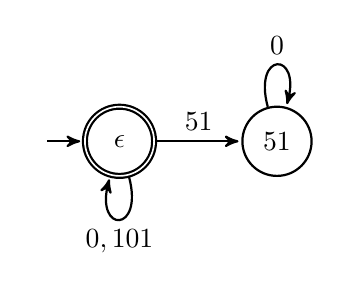
\begin{tikzpicture}
        [->,>=stealth',shorten >=1pt,auto,node distance=2cm,
        thick,base node/.style={circle,draw,minimum size=16pt}, real node/.style={double,circle,draw,minimum size=35pt}]
    
    
    
    \node[initial,initial text={}, accepting, state] (1) {$\epsilon$};
    \node[state](2)[right of=1 ]{$51$}[above];
    
    \path[]
    (1) edge [loop below]node {$0,101$} (1)
    (1) edge node {$51$} (2)
    (2) edge [loop above]node {$0$} (2);
    
    
    \end{tikzpicture}
    
    
    
    \end{document}